% Options for packages loaded elsewhere
\PassOptionsToPackage{unicode}{hyperref}
\PassOptionsToPackage{hyphens}{url}
%
\documentclass[
]{article}
\title{Class17}
\author{Gabrielle Meza (A13747395)}
\date{11/24/2021}

\usepackage{amsmath,amssymb}
\usepackage{lmodern}
\usepackage{iftex}
\ifPDFTeX
  \usepackage[T1]{fontenc}
  \usepackage[utf8]{inputenc}
  \usepackage{textcomp} % provide euro and other symbols
\else % if luatex or xetex
  \usepackage{unicode-math}
  \defaultfontfeatures{Scale=MatchLowercase}
  \defaultfontfeatures[\rmfamily]{Ligatures=TeX,Scale=1}
\fi
% Use upquote if available, for straight quotes in verbatim environments
\IfFileExists{upquote.sty}{\usepackage{upquote}}{}
\IfFileExists{microtype.sty}{% use microtype if available
  \usepackage[]{microtype}
  \UseMicrotypeSet[protrusion]{basicmath} % disable protrusion for tt fonts
}{}
\makeatletter
\@ifundefined{KOMAClassName}{% if non-KOMA class
  \IfFileExists{parskip.sty}{%
    \usepackage{parskip}
  }{% else
    \setlength{\parindent}{0pt}
    \setlength{\parskip}{6pt plus 2pt minus 1pt}}
}{% if KOMA class
  \KOMAoptions{parskip=half}}
\makeatother
\usepackage{xcolor}
\IfFileExists{xurl.sty}{\usepackage{xurl}}{} % add URL line breaks if available
\IfFileExists{bookmark.sty}{\usepackage{bookmark}}{\usepackage{hyperref}}
\hypersetup{
  pdftitle={Class17},
  pdfauthor={Gabrielle Meza (A13747395)},
  hidelinks,
  pdfcreator={LaTeX via pandoc}}
\urlstyle{same} % disable monospaced font for URLs
\usepackage[margin=1in]{geometry}
\usepackage{color}
\usepackage{fancyvrb}
\newcommand{\VerbBar}{|}
\newcommand{\VERB}{\Verb[commandchars=\\\{\}]}
\DefineVerbatimEnvironment{Highlighting}{Verbatim}{commandchars=\\\{\}}
% Add ',fontsize=\small' for more characters per line
\usepackage{framed}
\definecolor{shadecolor}{RGB}{248,248,248}
\newenvironment{Shaded}{\begin{snugshade}}{\end{snugshade}}
\newcommand{\AlertTok}[1]{\textcolor[rgb]{0.94,0.16,0.16}{#1}}
\newcommand{\AnnotationTok}[1]{\textcolor[rgb]{0.56,0.35,0.01}{\textbf{\textit{#1}}}}
\newcommand{\AttributeTok}[1]{\textcolor[rgb]{0.77,0.63,0.00}{#1}}
\newcommand{\BaseNTok}[1]{\textcolor[rgb]{0.00,0.00,0.81}{#1}}
\newcommand{\BuiltInTok}[1]{#1}
\newcommand{\CharTok}[1]{\textcolor[rgb]{0.31,0.60,0.02}{#1}}
\newcommand{\CommentTok}[1]{\textcolor[rgb]{0.56,0.35,0.01}{\textit{#1}}}
\newcommand{\CommentVarTok}[1]{\textcolor[rgb]{0.56,0.35,0.01}{\textbf{\textit{#1}}}}
\newcommand{\ConstantTok}[1]{\textcolor[rgb]{0.00,0.00,0.00}{#1}}
\newcommand{\ControlFlowTok}[1]{\textcolor[rgb]{0.13,0.29,0.53}{\textbf{#1}}}
\newcommand{\DataTypeTok}[1]{\textcolor[rgb]{0.13,0.29,0.53}{#1}}
\newcommand{\DecValTok}[1]{\textcolor[rgb]{0.00,0.00,0.81}{#1}}
\newcommand{\DocumentationTok}[1]{\textcolor[rgb]{0.56,0.35,0.01}{\textbf{\textit{#1}}}}
\newcommand{\ErrorTok}[1]{\textcolor[rgb]{0.64,0.00,0.00}{\textbf{#1}}}
\newcommand{\ExtensionTok}[1]{#1}
\newcommand{\FloatTok}[1]{\textcolor[rgb]{0.00,0.00,0.81}{#1}}
\newcommand{\FunctionTok}[1]{\textcolor[rgb]{0.00,0.00,0.00}{#1}}
\newcommand{\ImportTok}[1]{#1}
\newcommand{\InformationTok}[1]{\textcolor[rgb]{0.56,0.35,0.01}{\textbf{\textit{#1}}}}
\newcommand{\KeywordTok}[1]{\textcolor[rgb]{0.13,0.29,0.53}{\textbf{#1}}}
\newcommand{\NormalTok}[1]{#1}
\newcommand{\OperatorTok}[1]{\textcolor[rgb]{0.81,0.36,0.00}{\textbf{#1}}}
\newcommand{\OtherTok}[1]{\textcolor[rgb]{0.56,0.35,0.01}{#1}}
\newcommand{\PreprocessorTok}[1]{\textcolor[rgb]{0.56,0.35,0.01}{\textit{#1}}}
\newcommand{\RegionMarkerTok}[1]{#1}
\newcommand{\SpecialCharTok}[1]{\textcolor[rgb]{0.00,0.00,0.00}{#1}}
\newcommand{\SpecialStringTok}[1]{\textcolor[rgb]{0.31,0.60,0.02}{#1}}
\newcommand{\StringTok}[1]{\textcolor[rgb]{0.31,0.60,0.02}{#1}}
\newcommand{\VariableTok}[1]{\textcolor[rgb]{0.00,0.00,0.00}{#1}}
\newcommand{\VerbatimStringTok}[1]{\textcolor[rgb]{0.31,0.60,0.02}{#1}}
\newcommand{\WarningTok}[1]{\textcolor[rgb]{0.56,0.35,0.01}{\textbf{\textit{#1}}}}
\usepackage{longtable,booktabs,array}
\usepackage{calc} % for calculating minipage widths
% Correct order of tables after \paragraph or \subparagraph
\usepackage{etoolbox}
\makeatletter
\patchcmd\longtable{\par}{\if@noskipsec\mbox{}\fi\par}{}{}
\makeatother
% Allow footnotes in longtable head/foot
\IfFileExists{footnotehyper.sty}{\usepackage{footnotehyper}}{\usepackage{footnote}}
\makesavenoteenv{longtable}
\usepackage{graphicx}
\makeatletter
\def\maxwidth{\ifdim\Gin@nat@width>\linewidth\linewidth\else\Gin@nat@width\fi}
\def\maxheight{\ifdim\Gin@nat@height>\textheight\textheight\else\Gin@nat@height\fi}
\makeatother
% Scale images if necessary, so that they will not overflow the page
% margins by default, and it is still possible to overwrite the defaults
% using explicit options in \includegraphics[width, height, ...]{}
\setkeys{Gin}{width=\maxwidth,height=\maxheight,keepaspectratio}
% Set default figure placement to htbp
\makeatletter
\def\fps@figure{htbp}
\makeatother
\setlength{\emergencystretch}{3em} % prevent overfull lines
\providecommand{\tightlist}{%
  \setlength{\itemsep}{0pt}\setlength{\parskip}{0pt}}
\setcounter{secnumdepth}{-\maxdimen} % remove section numbering
\ifLuaTeX
  \usepackage{selnolig}  % disable illegal ligatures
\fi

\begin{document}
\maketitle

\begin{Shaded}
\begin{Highlighting}[]
\NormalTok{vax }\OtherTok{\textless{}{-}} \FunctionTok{read.csv}\NormalTok{(}\StringTok{"covid19vaccinesbyzipcode\_test.csv"}\NormalTok{)}
\FunctionTok{head}\NormalTok{(vax)}
\end{Highlighting}
\end{Shaded}

\begin{verbatim}
##   as_of_date zip_code_tabulation_area local_health_jurisdiction         county
## 1 2021-01-05                    92395            San Bernardino San Bernardino
## 2 2021-01-05                    93206                      Kern           Kern
## 3 2021-01-05                    91006               Los Angeles    Los Angeles
## 4 2021-01-05                    91901                 San Diego      San Diego
## 5 2021-01-05                    92230                 Riverside      Riverside
## 6 2021-01-05                    92662                    Orange         Orange
##   vaccine_equity_metric_quartile                 vem_source
## 1                              1 Healthy Places Index Score
## 2                              1 Healthy Places Index Score
## 3                              3 Healthy Places Index Score
## 4                              3 Healthy Places Index Score
## 5                              1 Healthy Places Index Score
## 6                              4 Healthy Places Index Score
##   age12_plus_population age5_plus_population persons_fully_vaccinated
## 1               35915.3                40888                       NA
## 2                1237.5                 1521                       NA
## 3               28742.7                31347                       19
## 4               15549.8                16905                       12
## 5                2320.2                 2526                       NA
## 6                2349.5                 2397                       NA
##   persons_partially_vaccinated percent_of_population_fully_vaccinated
## 1                           NA                                     NA
## 2                           NA                                     NA
## 3                          873                               0.000606
## 4                          271                               0.000710
## 5                           NA                                     NA
## 6                           NA                                     NA
##   percent_of_population_partially_vaccinated
## 1                                         NA
## 2                                         NA
## 3                                   0.027850
## 4                                   0.016031
## 5                                         NA
## 6                                         NA
##   percent_of_population_with_1_plus_dose
## 1                                     NA
## 2                                     NA
## 3                               0.028456
## 4                               0.016741
## 5                                     NA
## 6                                     NA
##                                                                redacted
## 1 Information redacted in accordance with CA state privacy requirements
## 2 Information redacted in accordance with CA state privacy requirements
## 3                                                                    No
## 4                                                                    No
## 5 Information redacted in accordance with CA state privacy requirements
## 6 Information redacted in accordance with CA state privacy requirements
\end{verbatim}

\begin{Shaded}
\begin{Highlighting}[]
\FunctionTok{colnames}\NormalTok{(vax)}
\end{Highlighting}
\end{Shaded}

\begin{verbatim}
##  [1] "as_of_date"                                
##  [2] "zip_code_tabulation_area"                  
##  [3] "local_health_jurisdiction"                 
##  [4] "county"                                    
##  [5] "vaccine_equity_metric_quartile"            
##  [6] "vem_source"                                
##  [7] "age12_plus_population"                     
##  [8] "age5_plus_population"                      
##  [9] "persons_fully_vaccinated"                  
## [10] "persons_partially_vaccinated"              
## [11] "percent_of_population_fully_vaccinated"    
## [12] "percent_of_population_partially_vaccinated"
## [13] "percent_of_population_with_1_plus_dose"    
## [14] "redacted"
\end{verbatim}

\begin{quote}
Q1. What column details the total number of people fully vaccinated?
\end{quote}

``persons\_fully\_vaccinated''

\begin{quote}
Q2. What column details the Zip code tabulation area?
\end{quote}

``zip\_code\_tabulation\_area''

\begin{quote}
Q3. What is the earliest date in this dataset?
\end{quote}

\begin{Shaded}
\begin{Highlighting}[]
\FunctionTok{min}\NormalTok{(vax}\SpecialCharTok{$}\NormalTok{as\_of\_date)}
\end{Highlighting}
\end{Shaded}

\begin{verbatim}
## [1] "2021-01-05"
\end{verbatim}

\begin{quote}
Q4. What is the latest date in this dataset?
\end{quote}

\begin{Shaded}
\begin{Highlighting}[]
\FunctionTok{max}\NormalTok{(vax}\SpecialCharTok{$}\NormalTok{as\_of\_date)}
\end{Highlighting}
\end{Shaded}

\begin{verbatim}
## [1] "2021-11-23"
\end{verbatim}

let's call the \textbf{skim()} function from the skimr package to get a
quick overview of this dataset:

\begin{Shaded}
\begin{Highlighting}[]
\NormalTok{skimr}\SpecialCharTok{::}\FunctionTok{skim}\NormalTok{(vax)}
\end{Highlighting}
\end{Shaded}

\begin{longtable}[]{@{}ll@{}}
\caption{Data summary}\tabularnewline
\toprule
\endhead
Name & vax \\
Number of rows & 82908 \\
Number of columns & 14 \\
\_\_\_\_\_\_\_\_\_\_\_\_\_\_\_\_\_\_\_\_\_\_\_ & \\
Column type frequency: & \\
character & 5 \\
numeric & 9 \\
\_\_\_\_\_\_\_\_\_\_\_\_\_\_\_\_\_\_\_\_\_\_\_\_ & \\
Group variables & None \\
\bottomrule
\end{longtable}

\textbf{Variable type: character}

\begin{longtable}[]{@{}lrrrrrrr@{}}
\toprule
skim\_variable & n\_missing & complete\_rate & min & max & empty &
n\_unique & whitespace \\
\midrule
\endhead
as\_of\_date & 0 & 1 & 10 & 10 & 0 & 47 & 0 \\
local\_health\_jurisdiction & 0 & 1 & 0 & 15 & 235 & 62 & 0 \\
county & 0 & 1 & 0 & 15 & 235 & 59 & 0 \\
vem\_source & 0 & 1 & 15 & 26 & 0 & 3 & 0 \\
redacted & 0 & 1 & 2 & 69 & 0 & 2 & 0 \\
\bottomrule
\end{longtable}

\textbf{Variable type: numeric}

\begin{longtable}[]{@{}
  >{\raggedright\arraybackslash}p{(\columnwidth - 20\tabcolsep) * \real{0.32}}
  >{\raggedleft\arraybackslash}p{(\columnwidth - 20\tabcolsep) * \real{0.08}}
  >{\raggedleft\arraybackslash}p{(\columnwidth - 20\tabcolsep) * \real{0.11}}
  >{\raggedleft\arraybackslash}p{(\columnwidth - 20\tabcolsep) * \real{0.07}}
  >{\raggedleft\arraybackslash}p{(\columnwidth - 20\tabcolsep) * \real{0.07}}
  >{\raggedleft\arraybackslash}p{(\columnwidth - 20\tabcolsep) * \real{0.05}}
  >{\raggedleft\arraybackslash}p{(\columnwidth - 20\tabcolsep) * \real{0.07}}
  >{\raggedleft\arraybackslash}p{(\columnwidth - 20\tabcolsep) * \real{0.07}}
  >{\raggedleft\arraybackslash}p{(\columnwidth - 20\tabcolsep) * \real{0.07}}
  >{\raggedleft\arraybackslash}p{(\columnwidth - 20\tabcolsep) * \real{0.07}}
  >{\raggedright\arraybackslash}p{(\columnwidth - 20\tabcolsep) * \real{0.05}}@{}}
\toprule
\begin{minipage}[b]{\linewidth}\raggedright
skim\_variable
\end{minipage} & \begin{minipage}[b]{\linewidth}\raggedleft
n\_missing
\end{minipage} & \begin{minipage}[b]{\linewidth}\raggedleft
complete\_rate
\end{minipage} & \begin{minipage}[b]{\linewidth}\raggedleft
mean
\end{minipage} & \begin{minipage}[b]{\linewidth}\raggedleft
sd
\end{minipage} & \begin{minipage}[b]{\linewidth}\raggedleft
p0
\end{minipage} & \begin{minipage}[b]{\linewidth}\raggedleft
p25
\end{minipage} & \begin{minipage}[b]{\linewidth}\raggedleft
p50
\end{minipage} & \begin{minipage}[b]{\linewidth}\raggedleft
p75
\end{minipage} & \begin{minipage}[b]{\linewidth}\raggedleft
p100
\end{minipage} & \begin{minipage}[b]{\linewidth}\raggedright
hist
\end{minipage} \\
\midrule
\endhead
zip\_code\_tabulation\_area & 0 & 1.00 & 93665.11 & 1817.39 & 90001 &
92257.75 & 93658.50 & 95380.50 & 97635.0 & ▃▅▅▇▁ \\
vaccine\_equity\_metric\_quartile & 4089 & 0.95 & 2.44 & 1.11 & 1 & 1.00
& 2.00 & 3.00 & 4.0 & ▇▇▁▇▇ \\
age12\_plus\_population & 0 & 1.00 & 18895.04 & 18993.94 & 0 & 1346.95 &
13685.10 & 31756.12 & 88556.7 & ▇▃▂▁▁ \\
age5\_plus\_population & 0 & 1.00 & 20875.24 & 21106.04 & 0 & 1460.50 &
15364.00 & 34877.00 & 101902.0 & ▇▃▂▁▁ \\
persons\_fully\_vaccinated & 8355 & 0.90 & 9585.35 & 11609.12 & 11 &
516.00 & 4210.00 & 16095.00 & 71219.0 & ▇▂▁▁▁ \\
persons\_partially\_vaccinated & 8355 & 0.90 & 1894.87 & 2105.55 & 11 &
198.00 & 1269.00 & 2880.00 & 20159.0 & ▇▁▁▁▁ \\
percent\_of\_population\_fully\_vaccinated & 8355 & 0.90 & 0.43 & 0.27 &
0 & 0.20 & 0.44 & 0.63 & 1.0 & ▇▆▇▆▂ \\
percent\_of\_population\_partially\_vaccinated & 8355 & 0.90 & 0.10 &
0.10 & 0 & 0.06 & 0.07 & 0.11 & 1.0 & ▇▁▁▁▁ \\
percent\_of\_population\_with\_1\_plus\_dose & 8355 & 0.90 & 0.51 & 0.26
& 0 & 0.31 & 0.53 & 0.71 & 1.0 & ▅▅▇▇▃ \\
\bottomrule
\end{longtable}

\begin{quote}
Q5. How many numeric columns are in this dataset?
\end{quote}

9

\begin{quote}
Q6. Note that there are ``missing values'' in the dataset. How many NA
values there in the persons\_fully\_vaccinated column?
\end{quote}

\begin{Shaded}
\begin{Highlighting}[]
\FunctionTok{sum}\NormalTok{( }\FunctionTok{is.na}\NormalTok{(vax}\SpecialCharTok{$}\NormalTok{persons\_fully\_vaccinated) )}
\end{Highlighting}
\end{Shaded}

\begin{verbatim}
## [1] 8355
\end{verbatim}

\begin{quote}
Q7. What percent of persons\_fully\_vaccinated values are missing (to 2
significant figures)?
\end{quote}

\begin{Shaded}
\begin{Highlighting}[]
\FunctionTok{nrow}\NormalTok{(vax)}
\end{Highlighting}
\end{Shaded}

\begin{verbatim}
## [1] 82908
\end{verbatim}

\begin{Shaded}
\begin{Highlighting}[]
\NormalTok{(}\DecValTok{8355}\SpecialCharTok{/} \DecValTok{82908}\NormalTok{) }\SpecialCharTok{*} \DecValTok{100}
\end{Highlighting}
\end{Shaded}

\begin{verbatim}
## [1] 10.07744
\end{verbatim}

One of the ``character'' columns of the data is as\_of\_date, which
contains dates in the Year-Month-Day format.

Dates and times can be annoying to work with at the best of times.
However, in R we have the excellent lubridate package, which can make
life allot easier. Here is a quick example to get you started:

\begin{Shaded}
\begin{Highlighting}[]
\FunctionTok{library}\NormalTok{(lubridate)}
\end{Highlighting}
\end{Shaded}

\begin{verbatim}
## 
## Attaching package: 'lubridate'
\end{verbatim}

\begin{verbatim}
## The following objects are masked from 'package:base':
## 
##     date, intersect, setdiff, union
\end{verbatim}

\begin{Shaded}
\begin{Highlighting}[]
\FunctionTok{today}\NormalTok{()}
\end{Highlighting}
\end{Shaded}

\begin{verbatim}
## [1] "2021-11-24"
\end{verbatim}

\begin{quote}
Q9. How many days have passed since the last update of the dataset?
\end{quote}

\begin{Shaded}
\begin{Highlighting}[]
\CommentTok{\# Specify that we are using the year{-}month{-}day format}
\NormalTok{vax}\SpecialCharTok{$}\NormalTok{as\_of\_date }\OtherTok{\textless{}{-}} \FunctionTok{ymd}\NormalTok{(vax}\SpecialCharTok{$}\NormalTok{as\_of\_date)}
\end{Highlighting}
\end{Shaded}

\begin{quote}
Q10. How many unique dates are in the dataset (i.e.~how many different
dates are detailed)?
\end{quote}

\begin{Shaded}
\begin{Highlighting}[]
\FunctionTok{today}\NormalTok{() }\SpecialCharTok{{-}}\NormalTok{ vax}\SpecialCharTok{$}\NormalTok{as\_of\_date[}\DecValTok{1}\NormalTok{]}
\end{Highlighting}
\end{Shaded}

\begin{verbatim}
## Time difference of 323 days
\end{verbatim}

In R we can use the \textbf{zipcodeR} package to make working with these
codes easier

\begin{Shaded}
\begin{Highlighting}[]
\FunctionTok{library}\NormalTok{(zipcodeR)}
\FunctionTok{geocode\_zip}\NormalTok{(}\StringTok{\textquotesingle{}92037\textquotesingle{}}\NormalTok{)}
\end{Highlighting}
\end{Shaded}

\begin{verbatim}
## # A tibble: 1 x 3
##   zipcode   lat   lng
##   <chr>   <dbl> <dbl>
## 1 92037    32.8 -117.
\end{verbatim}

Calculate the distance between the centroids of any two ZIP codes in
miles, e.g.

\begin{Shaded}
\begin{Highlighting}[]
\FunctionTok{zip\_distance}\NormalTok{(}\StringTok{\textquotesingle{}92037\textquotesingle{}}\NormalTok{,}\StringTok{\textquotesingle{}92109\textquotesingle{}}\NormalTok{)}
\end{Highlighting}
\end{Shaded}

\begin{verbatim}
##   zipcode_a zipcode_b distance
## 1     92037     92109     2.33
\end{verbatim}

More usefully, we can pull census data about ZIP code areas (including
median household income etc.

\begin{Shaded}
\begin{Highlighting}[]
\FunctionTok{reverse\_zipcode}\NormalTok{(}\FunctionTok{c}\NormalTok{(}\StringTok{\textquotesingle{}92037\textquotesingle{}}\NormalTok{, }\StringTok{"92109"}\NormalTok{) )}
\end{Highlighting}
\end{Shaded}

\begin{verbatim}
## # A tibble: 2 x 24
##   zipcode zipcode_type major_city post_office_city common_city_list county state
##   <chr>   <chr>        <chr>      <chr>                      <blob> <chr>  <chr>
## 1 92037   Standard     La Jolla   La Jolla, CA           <raw 20 B> San D~ CA   
## 2 92109   Standard     San Diego  San Diego, CA          <raw 21 B> San D~ CA   
## # ... with 17 more variables: lat <dbl>, lng <dbl>, timezone <chr>,
## #   radius_in_miles <dbl>, area_code_list <blob>, population <int>,
## #   population_density <dbl>, land_area_in_sqmi <dbl>,
## #   water_area_in_sqmi <dbl>, housing_units <int>,
## #   occupied_housing_units <int>, median_home_value <int>,
## #   median_household_income <int>, bounds_west <dbl>, bounds_east <dbl>,
## #   bounds_north <dbl>, bounds_south <dbl>
\end{verbatim}

\begin{quote}
How many unique zip code
\end{quote}

\begin{Shaded}
\begin{Highlighting}[]
\FunctionTok{length}\NormalTok{(}\FunctionTok{unique}\NormalTok{(vax}\SpecialCharTok{$}\NormalTok{zip\_code\_tabulation\_area))}
\end{Highlighting}
\end{Shaded}

\begin{verbatim}
## [1] 1764
\end{verbatim}

Subsetting can get tedious and complicated quickly. we will use the
\textbf{filter()} function to do our subsetting from now on. this uses
\textbf{dlypr()}

We want to focus in on the San Diego County

\begin{Shaded}
\begin{Highlighting}[]
\FunctionTok{library}\NormalTok{(dplyr)}
\end{Highlighting}
\end{Shaded}

\begin{verbatim}
## 
## Attaching package: 'dplyr'
\end{verbatim}

\begin{verbatim}
## The following objects are masked from 'package:stats':
## 
##     filter, lag
\end{verbatim}

\begin{verbatim}
## The following objects are masked from 'package:base':
## 
##     intersect, setdiff, setequal, union
\end{verbatim}

\begin{Shaded}
\begin{Highlighting}[]
\NormalTok{sd }\OtherTok{\textless{}{-}} \FunctionTok{filter}\NormalTok{(vax, county }\SpecialCharTok{==} \StringTok{"San Diego"}\NormalTok{)}
\end{Highlighting}
\end{Shaded}

\begin{Shaded}
\begin{Highlighting}[]
\FunctionTok{nrow}\NormalTok{(sd)}
\end{Highlighting}
\end{Shaded}

\begin{verbatim}
## [1] 5029
\end{verbatim}

\begin{quote}
Q11. How many distinct zip codes are listed for San Diego County?
\end{quote}

\begin{Shaded}
\begin{Highlighting}[]
\FunctionTok{length}\NormalTok{(}\FunctionTok{unique}\NormalTok{(sd}\SpecialCharTok{$}\NormalTok{zip\_code\_tabulation\_area))}
\end{Highlighting}
\end{Shaded}

\begin{verbatim}
## [1] 107
\end{verbatim}

\begin{quote}
Q12. What San Diego County Zip code area has the largest 12 + Population
in this dataset?
\end{quote}

\begin{Shaded}
\begin{Highlighting}[]
\FunctionTok{which.max}\NormalTok{(vax}\SpecialCharTok{$}\NormalTok{age12\_plus\_population)}
\end{Highlighting}
\end{Shaded}

\begin{verbatim}
## [1] 192
\end{verbatim}

\begin{Shaded}
\begin{Highlighting}[]
\NormalTok{vax}\SpecialCharTok{$}\NormalTok{zip\_code\_tabulation\_area[}\FunctionTok{which.max}\NormalTok{(vax}\SpecialCharTok{$}\NormalTok{age12\_plus\_population)]}
\end{Highlighting}
\end{Shaded}

\begin{verbatim}
## [1] 91331
\end{verbatim}

\begin{Shaded}
\begin{Highlighting}[]
\NormalTok{sd}\SpecialCharTok{$}\NormalTok{zip\_code\_tabulation\_area[}\FunctionTok{which.max}\NormalTok{(sd}\SpecialCharTok{$}\NormalTok{age12\_plus\_population)]}
\end{Highlighting}
\end{Shaded}

\begin{verbatim}
## [1] 92154
\end{verbatim}

More complicated subsetting

\begin{Shaded}
\begin{Highlighting}[]
\NormalTok{sd}\FloatTok{.20} \OtherTok{\textless{}{-}} \FunctionTok{filter}\NormalTok{(vax, county }\SpecialCharTok{==} \StringTok{"San Diego"}\NormalTok{, }
\NormalTok{       age5\_plus\_population }\SpecialCharTok{\textgreater{}} \DecValTok{20000}\NormalTok{)}

\FunctionTok{nrow}\NormalTok{(sd}\FloatTok{.20}\NormalTok{)}
\end{Highlighting}
\end{Shaded}

\begin{verbatim}
## [1] 3055
\end{verbatim}

\begin{quote}
Q13. what is the average vaccination rate of San Diego as of yesterday?
\end{quote}

\begin{Shaded}
\begin{Highlighting}[]
\NormalTok{sd.now }\OtherTok{\textless{}{-}} \FunctionTok{filter}\NormalTok{(vax, county}\SpecialCharTok{==}\StringTok{"San Diego"}\NormalTok{,}
\NormalTok{                 as\_of\_date}\SpecialCharTok{==}\StringTok{"2021{-}11{-}23"}\NormalTok{)}
\FunctionTok{head}\NormalTok{(sd.now)}
\end{Highlighting}
\end{Shaded}

\begin{verbatim}
##   as_of_date zip_code_tabulation_area local_health_jurisdiction    county
## 1 2021-11-23                    92120                 San Diego San Diego
## 2 2021-11-23                    91962                 San Diego San Diego
## 3 2021-11-23                    92155                 San Diego San Diego
## 4 2021-11-23                    92147                 San Diego San Diego
## 5 2021-11-23                    91913                 San Diego San Diego
## 6 2021-11-23                    92114                 San Diego San Diego
##   vaccine_equity_metric_quartile                 vem_source
## 1                              4 Healthy Places Index Score
## 2                              3 Healthy Places Index Score
## 3                             NA            No VEM Assigned
## 4                             NA            No VEM Assigned
## 5                              3 Healthy Places Index Score
## 6                              2 Healthy Places Index Score
##   age12_plus_population age5_plus_population persons_fully_vaccinated
## 1               26372.9                28414                    21234
## 2                1758.7                 2020                      948
## 3                 456.0                  456                       70
## 4                 518.0                  518                       NA
## 5               43514.7                50461                    37974
## 6               59050.7                64945                    43708
##   persons_partially_vaccinated percent_of_population_fully_vaccinated
## 1                         3198                               0.747308
## 2                          126                               0.469307
## 3                           20                               0.153509
## 4                           NA                                     NA
## 5                         6690                               0.752542
## 6                         6261                               0.673000
##   percent_of_population_partially_vaccinated
## 1                                   0.112550
## 2                                   0.062376
## 3                                   0.043860
## 4                                         NA
## 5                                   0.132578
## 6                                   0.096405
##   percent_of_population_with_1_plus_dose
## 1                               0.859858
## 2                               0.531683
## 3                               0.197369
## 4                                     NA
## 5                               0.885120
## 6                               0.769405
##                                                                redacted
## 1                                                                    No
## 2                                                                    No
## 3                                                                    No
## 4 Information redacted in accordance with CA state privacy requirements
## 5                                                                    No
## 6                                                                    No
\end{verbatim}

\begin{Shaded}
\begin{Highlighting}[]
\NormalTok{sd.now}\SpecialCharTok{$}\NormalTok{percent\_of\_population\_fully\_vaccinated}
\end{Highlighting}
\end{Shaded}

\begin{verbatim}
##   [1] 0.747308 0.469307 0.153509       NA 0.752542 0.673000 0.171930 0.628913
##   [9] 0.355234 0.686848 0.496899 0.694990 0.725720 0.576161 0.652680 0.806525
##  [17] 0.718495 1.000000 0.633126 0.835713 0.855294 0.657697 0.631422 0.846959
##  [25] 0.769692 1.000000       NA 0.628480 0.844500       NA 0.683163 0.523179
##  [33] 0.082372 0.771474 0.464088 0.592998 0.651956 0.632170 0.571643 0.656561
##  [41] 0.603904 0.626561 0.691278 0.723539 0.813734 0.707481 0.730845 0.617369
##  [49] 0.841184 0.743946 0.759115 1.000000 0.676833 0.944622 0.667700 0.638762
##  [57] 0.766287 1.000000 0.711136 0.743590 0.798508 0.916196 0.694622 0.613783
##  [65] 0.526130 0.641578 0.700739 0.484584 0.370307 0.594036 0.618409 0.682470
##  [73] 0.863395 0.840959 1.000000 0.249635 0.610675 1.000000 0.729044 0.614751
##  [81] 0.586075 0.699525 1.000000 0.769195 0.715999 0.670258 1.000000 0.521976
##  [89] 0.010726 0.732941 0.632636 0.559401 0.010169 0.639952 0.891644 0.713647
##  [97] 0.672947 0.653994 0.569850 0.665486 0.523125 0.673358 0.951807 0.604313
## [105] 0.744649 0.787222 0.894858
\end{verbatim}

\begin{Shaded}
\begin{Highlighting}[]
\FunctionTok{summary}\NormalTok{(sd.now}\SpecialCharTok{$}\NormalTok{percent\_of\_population\_fully\_vaccinated)}
\end{Highlighting}
\end{Shaded}

\begin{verbatim}
##    Min. 1st Qu.  Median    Mean 3rd Qu.    Max.    NA's 
## 0.01017 0.61301 0.67965 0.67400 0.76932 1.00000       3
\end{verbatim}

\begin{quote}
Q14. Using either ggplot or base R graphics make a summary figure that
shows the distribution of Percent of Population Fully Vaccinated values
as of ``2021-11-09''? As a histogram
\end{quote}

\begin{Shaded}
\begin{Highlighting}[]
\FunctionTok{hist}\NormalTok{(sd.now}\SpecialCharTok{$}\NormalTok{percent\_of\_population\_fully\_vaccinated)}
\end{Highlighting}
\end{Shaded}

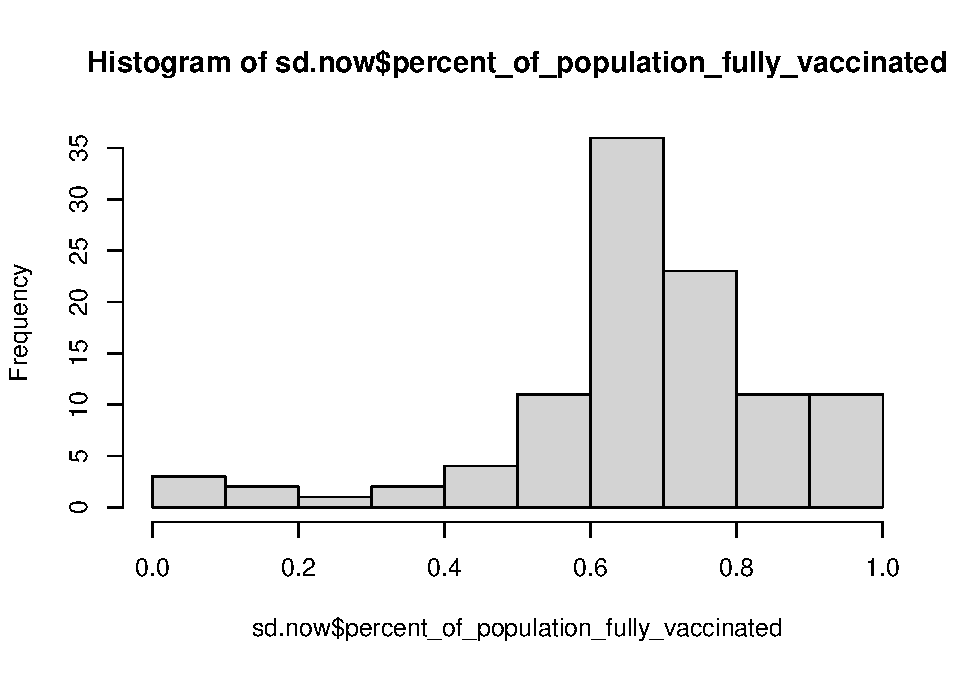
\includegraphics{Class17_Vax_files/figure-latex/unnamed-chunk-24-1.pdf}

This plot above is going to be susceptible to being skewed by ZIP code
areas with small populations. these will have big effects for just a
small number of unvax-ed folks\ldots{}

Now focus on UCSD/La Jolla area

\begin{quote}
Q. What is the population of the 92037 ZIP code area?
\end{quote}

\begin{Shaded}
\begin{Highlighting}[]
\NormalTok{ucsd }\OtherTok{\textless{}{-}} \FunctionTok{filter}\NormalTok{(sd.now, zip\_code\_tabulation\_area}\SpecialCharTok{==}\StringTok{"92037"}\NormalTok{)}
\NormalTok{ucsd}\SpecialCharTok{$}\NormalTok{age5\_plus\_population}
\end{Highlighting}
\end{Shaded}

\begin{verbatim}
## [1] 36144
\end{verbatim}

\begin{quote}
Q. What is the average vaccination value for this UCSD/La Jolla ZIP code
area?
\end{quote}

\begin{Shaded}
\begin{Highlighting}[]
\NormalTok{ucsd}\SpecialCharTok{$}\NormalTok{percent\_of\_population\_fully\_vaccinated}
\end{Highlighting}
\end{Shaded}

\begin{verbatim}
## [1] 0.916196
\end{verbatim}

\begin{quote}
Lets do my zipcode! 92124 and then where i am going: 92065
\end{quote}

\begin{Shaded}
\begin{Highlighting}[]
\NormalTok{tierrasanta}\OtherTok{\textless{}{-}} \FunctionTok{filter}\NormalTok{(sd.now, zip\_code\_tabulation\_area}\SpecialCharTok{==}\StringTok{"92124"}\NormalTok{)}
\NormalTok{tierrasanta}\SpecialCharTok{$}\NormalTok{age5\_plus\_population}
\end{Highlighting}
\end{Shaded}

\begin{verbatim}
## [1] 29040
\end{verbatim}

\begin{Shaded}
\begin{Highlighting}[]
\NormalTok{tierrasanta}\SpecialCharTok{$}\NormalTok{percent\_of\_population\_fully\_vaccinated}
\end{Highlighting}
\end{Shaded}

\begin{verbatim}
## [1] 0.559401
\end{verbatim}

\begin{Shaded}
\begin{Highlighting}[]
\NormalTok{ramona }\OtherTok{\textless{}{-}} \FunctionTok{filter}\NormalTok{(sd.now, zip\_code\_tabulation\_area}\SpecialCharTok{==}\StringTok{"92065"}\NormalTok{)}
\NormalTok{ramona}\SpecialCharTok{$}\NormalTok{percent\_of\_population\_fully\_vaccinated}
\end{Highlighting}
\end{Shaded}

\begin{verbatim}
## [1] 0.52613
\end{verbatim}

Lets make a time series of vacination rate for a given ZIP code area. I
will do 92124

\begin{Shaded}
\begin{Highlighting}[]
\NormalTok{ttown }\OtherTok{\textless{}{-}} \FunctionTok{filter}\NormalTok{(vax, zip\_code\_tabulation\_area }\SpecialCharTok{==} \StringTok{"92124"}\NormalTok{)}
\FunctionTok{library}\NormalTok{(ggplot2)}
\end{Highlighting}
\end{Shaded}

\begin{Shaded}
\begin{Highlighting}[]
\FunctionTok{ggplot}\NormalTok{(ttown) }\SpecialCharTok{+} 
  \FunctionTok{aes}\NormalTok{(}\AttributeTok{x=}\NormalTok{as\_of\_date, }\AttributeTok{y=}\NormalTok{percent\_of\_population\_fully\_vaccinated) }\SpecialCharTok{+} 
  \FunctionTok{geom\_point}\NormalTok{() }\SpecialCharTok{+}
  \FunctionTok{labs}\NormalTok{(}\AttributeTok{x=}\StringTok{"Date"}\NormalTok{, }\AttributeTok{y=}\StringTok{"Percent Vaccinated"}\NormalTok{)}
\end{Highlighting}
\end{Shaded}

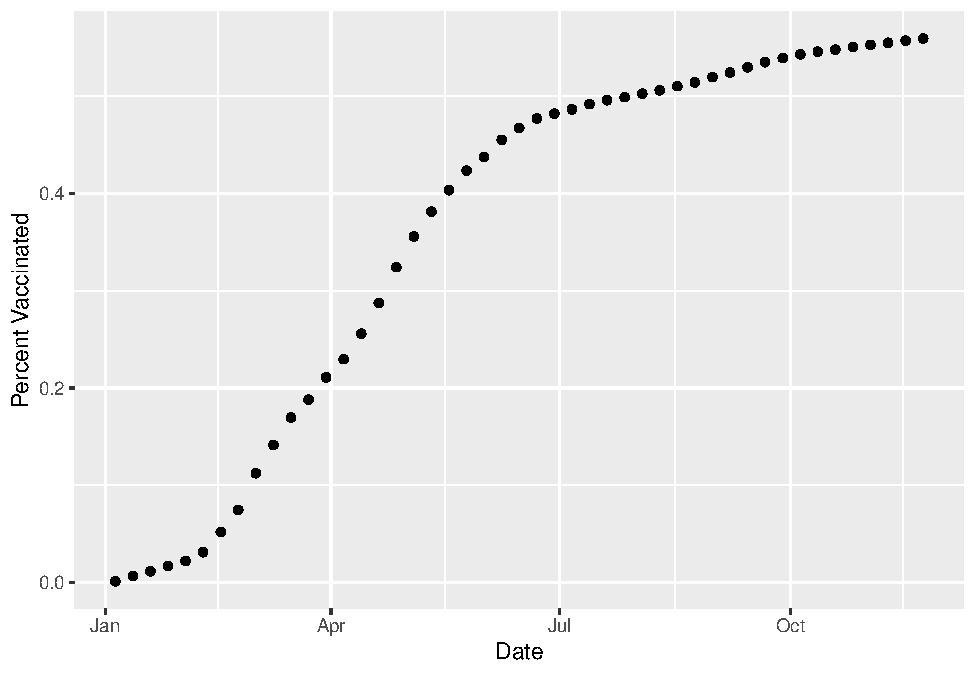
\includegraphics{Class17_Vax_files/figure-latex/unnamed-chunk-30-1.pdf}

Let's make this plot for all of SD county zip codes that have a
population as large as 92037 (UCSD)

\begin{Shaded}
\begin{Highlighting}[]
\NormalTok{sd}\FloatTok{.36} \OtherTok{\textless{}{-}} \FunctionTok{filter}\NormalTok{(vax, county}\SpecialCharTok{==}\StringTok{"San Diego"}\NormalTok{,}
\NormalTok{                age5\_plus\_population }\SpecialCharTok{\textgreater{}} \DecValTok{36144}\NormalTok{)}
\FunctionTok{head}\NormalTok{(sd}\FloatTok{.36}\NormalTok{)}
\end{Highlighting}
\end{Shaded}

\begin{verbatim}
##   as_of_date zip_code_tabulation_area local_health_jurisdiction    county
## 1 2021-01-05                    92058                 San Diego San Diego
## 2 2021-01-05                    92078                 San Diego San Diego
## 3 2021-01-05                    92019                 San Diego San Diego
## 4 2021-01-05                    92117                 San Diego San Diego
## 5 2021-01-05                    92057                 San Diego San Diego
## 6 2021-01-05                    91913                 San Diego San Diego
##   vaccine_equity_metric_quartile                 vem_source
## 1                              1 Healthy Places Index Score
## 2                              3 Healthy Places Index Score
## 3                              3 Healthy Places Index Score
## 4                              3 Healthy Places Index Score
## 5                              2 Healthy Places Index Score
## 6                              3 Healthy Places Index Score
##   age12_plus_population age5_plus_population persons_fully_vaccinated
## 1               34956.0                39695                       NA
## 2               41789.5                47476                       37
## 3               37439.4                40464                       25
## 4               50041.6                53839                       42
## 5               51927.0                56906                       22
## 6               43514.7                50461                       37
##   persons_partially_vaccinated percent_of_population_fully_vaccinated
## 1                           NA                                     NA
## 2                          688                               0.000779
## 3                          610                               0.000618
## 4                         1143                               0.000780
## 5                          691                               0.000387
## 6                         1993                               0.000733
##   percent_of_population_partially_vaccinated
## 1                                         NA
## 2                                   0.014492
## 3                                   0.015075
## 4                                   0.021230
## 5                                   0.012143
## 6                                   0.039496
##   percent_of_population_with_1_plus_dose
## 1                                     NA
## 2                               0.015271
## 3                               0.015693
## 4                               0.022010
## 5                               0.012530
## 6                               0.040229
##                                                                redacted
## 1 Information redacted in accordance with CA state privacy requirements
## 2                                                                    No
## 3                                                                    No
## 4                                                                    No
## 5                                                                    No
## 6                                                                    No
\end{verbatim}

\begin{quote}
Lets do a plot for all of california, with similar populations.
Populations bigger than UCSD: 36144
\end{quote}

\begin{Shaded}
\begin{Highlighting}[]
\NormalTok{ca }\OtherTok{\textless{}{-}} \FunctionTok{filter}\NormalTok{(vax, age5\_plus\_population }\SpecialCharTok{\textgreater{}} \DecValTok{36144}\NormalTok{)}
\end{Highlighting}
\end{Shaded}

How many zip codes withth is pop?

\begin{Shaded}
\begin{Highlighting}[]
\FunctionTok{length}\NormalTok{(}\FunctionTok{unique}\NormalTok{(ca}\SpecialCharTok{$}\NormalTok{zip\_code\_tabulation\_area))}
\end{Highlighting}
\end{Shaded}

\begin{verbatim}
## [1] 411
\end{verbatim}

Now lets make the plot

\begin{Shaded}
\begin{Highlighting}[]
\FunctionTok{ggplot}\NormalTok{(ca) }\SpecialCharTok{+} 
  \FunctionTok{aes}\NormalTok{(}\AttributeTok{x=}\NormalTok{as\_of\_date, }\AttributeTok{y=}\NormalTok{percent\_of\_population\_fully\_vaccinated, }
      \AttributeTok{group=}\NormalTok{zip\_code\_tabulation\_area) }\SpecialCharTok{+}
  \FunctionTok{geom\_line}\NormalTok{(}\AttributeTok{alpjha=}\FloatTok{0.2}\NormalTok{) }\SpecialCharTok{+}
  \FunctionTok{labs}\NormalTok{(}\AttributeTok{x=}\StringTok{"Date"}\NormalTok{, }\AttributeTok{y=}\StringTok{"Percent Vaccinated"}\NormalTok{)}
\end{Highlighting}
\end{Shaded}

\begin{verbatim}
## Warning: Ignoring unknown parameters: alpjha
\end{verbatim}

\begin{verbatim}
## Warning: Removed 176 row(s) containing missing values (geom_path).
\end{verbatim}

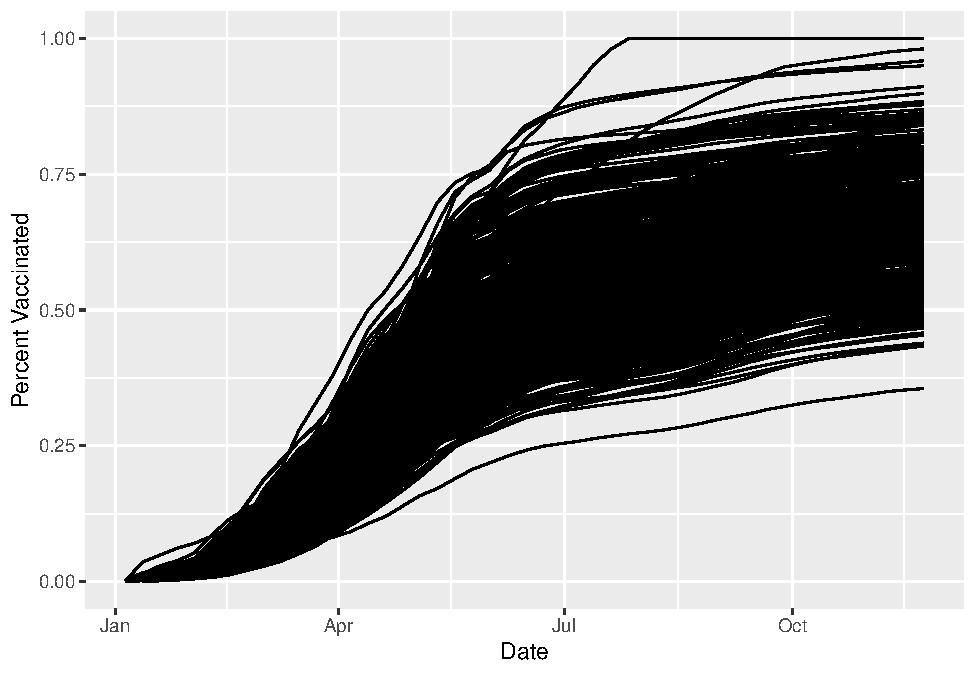
\includegraphics{Class17_Vax_files/figure-latex/unnamed-chunk-34-1.pdf}

What is the mean across the state for these 36k+ population areas?

\begin{Shaded}
\begin{Highlighting}[]
\NormalTok{ca.now }\OtherTok{\textless{}{-}} \FunctionTok{filter}\NormalTok{(ca, as\_of\_date}\SpecialCharTok{==}\StringTok{"2021{-}11{-}22"}\NormalTok{)}
\FunctionTok{summary}\NormalTok{(ca.now}\SpecialCharTok{$}\NormalTok{percent\_of\_population\_fully\_vaccinated)}
\end{Highlighting}
\end{Shaded}

\begin{verbatim}
##    Min. 1st Qu.  Median    Mean 3rd Qu.    Max. 
## 
\end{verbatim}

Add a line for the mean \% of people vaccinated in California.

\begin{Shaded}
\begin{Highlighting}[]
 \FunctionTok{ggplot}\NormalTok{(ca) }\SpecialCharTok{+} 
  \FunctionTok{aes}\NormalTok{(}\AttributeTok{x=}\NormalTok{as\_of\_date, }\AttributeTok{y=}\NormalTok{percent\_of\_population\_fully\_vaccinated, }
      \AttributeTok{group=}\NormalTok{zip\_code\_tabulation\_area) }\SpecialCharTok{+}
  \FunctionTok{geom\_line}\NormalTok{(}\AttributeTok{alpjha=}\FloatTok{0.2}\NormalTok{) }\SpecialCharTok{+}
  \FunctionTok{labs}\NormalTok{(}\AttributeTok{x=}\StringTok{"Date"}\NormalTok{, }\AttributeTok{y=}\StringTok{"Percent Vaccinated"}\NormalTok{) }\SpecialCharTok{+}
  \FunctionTok{geom\_hline}\NormalTok{(}\AttributeTok{yintercept =} \FloatTok{0.67}\NormalTok{, }\AttributeTok{color =} \StringTok{"Red"}\NormalTok{)}
\end{Highlighting}
\end{Shaded}

\begin{verbatim}
## Warning: Ignoring unknown parameters: alpjha
\end{verbatim}

\begin{verbatim}
## Warning: Removed 176 row(s) containing missing values (geom_path).
\end{verbatim}

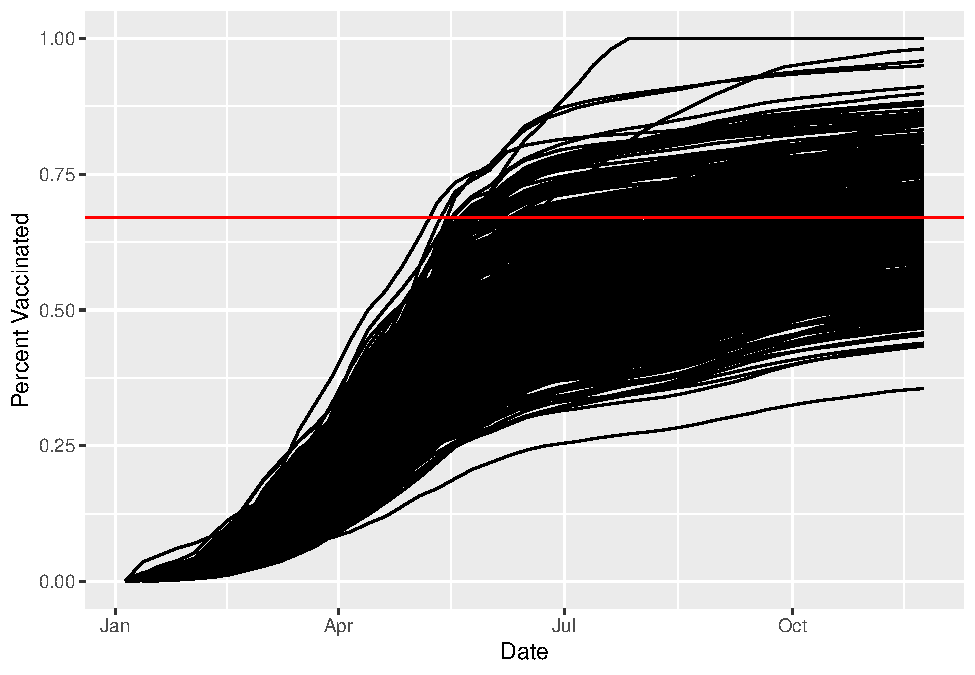
\includegraphics{Class17_Vax_files/figure-latex/unnamed-chunk-36-1.pdf}

\end{document}
